
\documentclass[journal,12pt,twocolumn]{IEEEtran}
\usepackage{graphicx}
\begin{document}

\title{Assignment Report: Implementing a Music Player}
\author{Advait Jain \\ CS22BTECH11003}
\date{May 18, 2023}

\maketitle

\section{Introduction}
The purpose of this assignment was to implement a music player using the Pygame library in Python. The music player allows users to play, pause, skip to the next song, and go back to the previous song. Additionally, the playlist is shuffled after reaching the end and a seek is provided to keep a track of the song played.

\section{Implementation}
The music player implementation consists of the following key components:
\begin{itemize}
  \item Pygame Initialization: The Pygame library is initialized to set up the game window and other necessary configurations.
  \item Window and Buttons: The game window is set up with buttons for previous, play/pause, and next functionalities. The buttons are defined using Pygame's Rect class.
  \item Playlist and Shuffling: The playlist is loaded from a specified directory, and the songs are shuffled using the random library. The current song index is tracked, along with a list of previous and popped songs for navigation. 
  \item Play Current Song: A function is defined to play the current song using the \texttt{pygame.mixer.music} module.
  \item Event Loop: The main event loop is responsible for handling user input, such as mouse clicks on buttons, and managing the playback state of the music player. It also autoplays the next song when the current song ends.
  \item Button Colors and Texts: The button colors and texts are updated based on user interaction and mouse hover.
  \item Displaying Current Song: The name of the current song being played is displayed on the screen using Pygame's font rendering capabilities. Also, a seek is implemented by using mutagen library.
  \end{itemize}
  \begin{figure}[ht]
		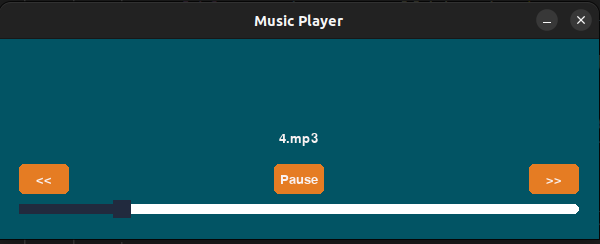
\includegraphics[width=0.3\linewidth]{UI/UI1.png}
		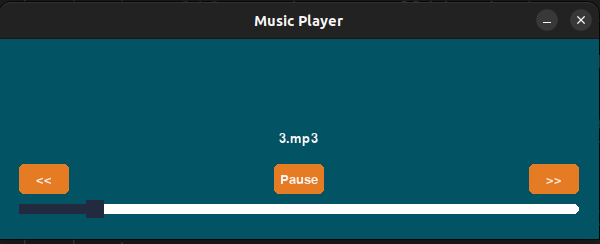
\includegraphics[width=0.3\linewidth]{UI/UI2.png}
		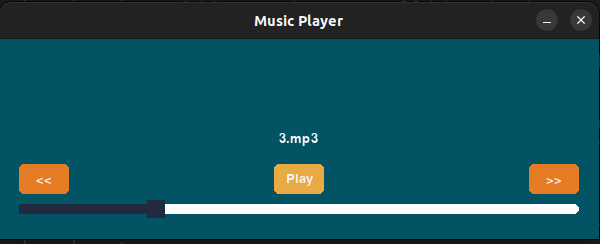
\includegraphics[width=0.3\linewidth]{UI/UI3.png}
\end{figure}
\section{Results and Observations}
The implemented music player successfully provides basic functionalities for playing, pausing, and navigating through songs. The playlist shuffling after reaching the end adds variation and keeps the listening experience fresh. The display of the current song name allows users to know the song that is currently playing.

\section{Limitations and Future Improvements}
\begin{itemize}
  \item The music player currently supports audio files in a specific directory only. Future improvements could involve adding support for different file formats and a more flexible file selection mechanism.
  \item The user interface could be enhanced by adding additional features such as a progress bar, volume control, and a visual representation of the music playback.
  \item Error handling and edge cases could be further addressed to ensure smooth and reliable functionality.
\end{itemize}

\section{Conclusion}
In conclusion, the implemented music player provides a basic yet functional user interface for playing and managing a playlist of songs. The assignment helped enhance programming skills in Python, particularly in using the Pygame library for graphical applications. Through this assignment, valuable experience was gained in event handling, button interaction, audio playback, and UI design.

Overall, the music player implementation successfully meets the assignment requirements and demonstrates a fundamental understanding of building interactive applications using Pygame.

\end{document}

